\documentclass[10pt,twocolumn,a4paper]{article}

\usepackage[utf8]{inputenc}
\usepackage[T1]{fontenc}
\usepackage{times}
\usepackage{graphicx}
\graphicspath{{figures/}}
\usepackage{amsmath}
\usepackage{amssymb}
\usepackage{geometry}
\usepackage{url}

\geometry{
	a4paper,
	left=1.6cm,
	right=1.6cm,
	top=1.8cm,
	bottom=2.0cm,
	columnsep=0.7cm
}

\setlength{\parindent}{0.35cm}
\setlength{\parskip}{0pt}

\title{\textbf{TennisVision: Player, Ball and Court Analysis in Broadcast Tennis Videos with YOLO26}}

\author{
	Student Name Surname 1\\
	Bachelor's Degree Programme in Applied Computer Science and Artificial Intelligence (ACSAI)\\
	Course: AI-LAB -- Computer Vision, Signal Processing, and Natural Language Processing\\
	Department of Computer Science, Sapienza University of Rome\\
	Matricola: XXXXXXX\\
	\texttt{student1@studenti.uniroma1.it}
}

\date{}

\begin{document}

	\maketitle

	\begin{abstract}
		This report presents TennisVision, a computer vision pipeline that analyzes broadcast tennis videos and automatically produces match statistics: shot count, shot speed, and player movement speed, rendered on an annotated video with a top-down minimap. The system combines three YOLO26-based components: a pose model trained to localize 14 court keypoints, a pretrained detector with built-in tracking for the two players, and a detector fine-tuned on a dedicated dataset for the tennis ball. Court keypoints are used to estimate a homography that maps image pixels to metric court coordinates, so that all speeds and distances are computed directly in meters without ad-hoc conversion factors. The raw ball track is refined with a piecewise parabolic smoother that removes outliers and bridges missed detections, and shots are detected as reversals of the ball motion along the court length. The fine-tuned ball detector reaches 0.90 mAP@50 on a held-out test set, and the court keypoint model is evaluated on more than two thousand unseen frames. The main contribution is the design and evaluation of the complete metric pipeline, together with the dataset preparation and fine-tuning of the two custom models.
	\end{abstract}

	\noindent\textbf{Keywords:} computer vision; object detection; pose estimation; YOLO; homography; sports video analysis.

	\section{Introduction}

	Quantitative match statistics such as shot speed, rally length, and player movement are a central tool in modern tennis coaching and broadcasting. Professional systems (e.g.\ Hawk-Eye) rely on multiple calibrated high-speed cameras and are not accessible to amateur players or analysts. The problem addressed by this project is the extraction of such statistics from a \emph{single} ordinary broadcast video, with no camera calibration and no manual annotation.

	The problem is challenging for several reasons. The ball is a small, fast, motion-blurred object that frequently disappears for several frames; the camera view is perspective-distorted, so pixel displacements do not translate directly into physical speeds; and broadcast footage contains distractors (line judges, ball kids, on-screen graphics) that confuse generic detectors. Existing open implementations typically address only one of these sub-problems, such as ball tracking with TrackNet~\cite{huang2019tracknet}, or rely on classical line-detection heuristics for the court that are fragile under varying surfaces and lighting.

	This project builds a complete pipeline on top of the modern YOLO26 family~\cite{ultralytics_yolo}. The personal contributions are: (i) the preparation of a 14-keypoint court dataset in Ultralytics pose format, including the remapping of the source annotation order to a canonical metric court model, and the training of a YOLO26-pose court detector; (ii) the fine-tuning and comparison of two YOLO26 variants (nano and small) on a dedicated tennis-ball dataset; (iii) a piecewise parabolic ball-trajectory smoother designed around the physics of ball flight, used instead of a generic recursive filter; (iv) shot- and bounce-detection rules operating in metric court space and image space respectively; and (v) the integration of all components into a single reproducible pipeline with metric analytics and visualization.

	The rest of the report is organized as follows. Section~2 reviews related work. Section~3 describes the pipeline. Section~4 presents the datasets, the training protocol, the results, and a critical discussion. Section~5 concludes the report.

	\section{Related Work}

	\textbf{Object detection.} Single-stage detectors of the YOLO family~\cite{redmon2016yolo} reformulate detection as a single regression pass over the image and remain the standard choice for real-time applications. This project uses YOLO26~\cite{ultralytics_yolo}, the most recent Ultralytics release, both as a pretrained person detector and as the backbone fine-tuned for ball detection; the underlying convolutional design descends from residual architectures~\cite{he2016resnet}. Pretrained weights come from large-scale benchmarks such as COCO~\cite{lin2014coco}, which include the \emph{person} and \emph{sports ball} classes; however, as shown in Section~4, the generic \emph{sports ball} class is insufficient for broadcast tennis footage, which motivates fine-tuning.

	\textbf{Ball tracking in sport video.} TrackNet~\cite{huang2019tracknet} introduced a heatmap-based deep network for tracking small, fast balls in sports broadcasts, demonstrating that learned detectors outperform color/shape heuristics. Compared to TrackNet, this project uses a general-purpose detector fine-tuned on tennis data, and moves the temporal reasoning into an explicit physics-motivated smoothing step, which is simpler to train and easier to inspect.

	\textbf{Court registration.} Mapping the broadcast view to a canonical court model is a planar homography estimation problem~\cite{hartley2004mvg}. Classical approaches detect court lines with edge/Hough heuristics and match them to the model; they are sensitive to surface color and lighting. Recent work replaces line detection with learned keypoint regression. This project follows the learned approach: a YOLO26-pose model regresses 14 court keypoints directly, and the homography is estimated from the detected points with RANSAC.

	Compared to the cited works and to existing tutorial repositories, the distinguishing element of this project is the fully \emph{metric} formulation: every downstream quantity (shot speed, player speed, shot detection) is computed in real-world meters after homography projection, which removes perspective bias from all statistics.

	\section{Methodology}

	The complete pipeline is shown in Fig.~\ref{fig:architecture}. It processes the input video in stages: court keypoint detection, homography estimation, player tracking, ball detection, trajectory smoothing, projection to metric court space, shot detection, statistics computation, and rendering.

\begin{figure*}[t]
	\centering
	
\includegraphics[width=0.95\textwidth]{02-PipelineDiagram.png}
	\caption{TennisVision pipeline. The input video is processed by three YOLO26 models: a pose model for the 14 court keypoints (from which the image-to-court homography is estimated), the pretrained detector with BoT-SORT association for the two players, and a fine-tuned detector for the ball. Ball detections are refined by a piecewise parabolic smoother, all positions are projected to metric court coordinates, shots are detected as motion reversals along the court length, and statistics are rendered on the annotated output video with a top-down minimap.}
	\label{fig:architecture}
\end{figure*}

	\textbf{Court keypoints and homography.} A YOLO26-pose model is trained to regress 14 keypoints corresponding to the intersections of the court lines (corners of the doubles and singles court, service boxes, and center marks). The canonical court model uses official ITF dimensions (doubles width $10.97$\,m, length $23.77$\,m), with the origin in the top-left corner and axes oriented as in image coordinates. The homography $H$ between detected image keypoints and their metric model positions is estimated with RANSAC. Keypoints are detected on \emph{every} frame, which doubles as a court/no-court classifier: broadcast footage cuts away to close-ups and replays, and frames with fewer than 4 confident keypoints are excluded from all later stages. Since the main broadcast camera is essentially static during rallies, a single homography is then estimated from the median of the keypoints over the court-visible frames, which suppresses per-frame jitter better than per-frame re-estimation. $H$ and $H^{-1}$ give the bidirectional pixel--meter mapping used by all later stages.

	\textbf{Player tracking.} The two players are detected with the pretrained YOLO26x person class and associated across frames by the tracker built into the Ultralytics framework. Among the tracked persons, the two players are selected as the two track IDs that spend the largest fraction of frames standing \emph{inside} the court after projection through $H$ -- a criterion robust to ball kids, line judges and spectators, who stand outside the playable area; the court half then only assigns the labels (player 1 near the camera, player 2 on the far side). Track IDs do not survive camera cuts, so the selection is repeated independently within each contiguous court-visible segment. The foot point of each bounding box is projected through $H$ to obtain the player position in meters.

	\textbf{Ball detection and smoothing.} The ball is detected by a YOLO26 model fine-tuned on a single-class tennis-ball dataset (Section~4.1). Raw detections are noisy: false positives (e.g.\ white shoes, second balls near the fence) and gaps of several frames are common. Instead of a recursive filter, a piecewise parabolic smoother is used, motivated by the observation that between two consecutive hits or bounces the ball trajectory is, to good approximation, a parabola in time even in image space. The smoother (i) gates outliers whose implied displacement from the last accepted point is physically impossible, (ii) splits the track into segments at sharp direction changes (hits, bounces) and long detection gaps, and (iii) fits a robust quadratic $x(t)$, $y(t)$ per segment by least squares with one outlier-trimming refit pass, evaluating the fit on every frame of the segment, which also bridges missed detections. Smoothed positions are then projected to court space.

	\textbf{Shot detection and analytics.} Working in court coordinates makes shot detection simple and robust: a hit is a reversal of the ball velocity along the court length ($y$ axis), i.e.\ a sign change of $\dot y$ after a short moving-average smoothing, subject to a minimum speed and a minimum temporal gap between consecutive hits. The projected position of a ball high above the court is displaced towards the far side, which can produce spurious mid-flight reversals; a reversal is therefore kept only if the ball lies close to a player's bounding box \emph{in the image} -- at the racquet the ball overlaps the player in pixels regardless of its height, whereas in court meters the height-induced offset can reach several meters -- and consecutive reversals attributed to the same player within a short interval are deduplicated. Each shot is attributed to the player closest to the ball in court space at the moment of the hit, and classified geometrically from the striker's metric position at the hit: a rally-opening hit struck from at or behind the baseline is a \emph{serve}, a hit struck between the net and the service line is a \emph{volley}, and everything else is a \emph{groundstroke} -- a classification that costs nothing because the positions are already in court coordinates. Ground bounces are detected separately, with a complementary signature in \emph{image} space: gravity acts along the image vertical, so a bounce is a falling-to-rising reversal of the vertical pixel velocity that is not explained by a player strike (reversals close in time to a detected hit, or close in court space to either player, are rejected). The bounce instant is also the only moment when the ball lies on the court plane, hence the only moment when the homography returns its exact metric position -- bounce locations are therefore the reliable anchor for in/out reasoning. Because positions are in meters, shot speed (km/h) and the per-frame player movement speed (computed over a 0.5\,s window to suppress projection jitter) need no pixel-to-meter conversion factor. Results are rendered as an annotated video: player and ball boxes with their detection confidence, the fitted parabolic trajectory drawn as a fading trail behind the ball, a top-down minimap of the court, and a statistics panel reporting, per player, the live shot count, last shot speed and type, average shot speed, and current movement speed.

	\textbf{Reused vs.\ original components.} The YOLO26 architecture, the pretrained weights, and the built-in tracker are taken from the Ultralytics framework~\cite{ultralytics_yolo} and used unmodified. The student's own contributions are the court-pose dataset conversion and keypoint remapping, the training of the court model and the fine-tuning of the ball models, the parabolic smoother, the metric shot/bounce-detection and analytics modules, and the overall pipeline integration.

	\section{Experimental Setup}

	Two models were trained: the ball detector (locally) and the court keypoint model (on Google Colab). Both are evaluated on held-out data.

	\subsection{Dataset}

	\textbf{Ball dataset.} A single-class tennis-ball detection dataset of 578 broadcast frames with bounding-box annotations, split into 428 training, 100 validation, and 50 test images. Images come from broadcast footage, so the ball is typically only a few pixels wide and often motion-blurred, which is the main source of difficulty. The dataset was used with its original split.

	\textbf{Court keypoint dataset.} A dataset of $1280\times720$ broadcast frames annotated with 14 court keypoints each, provided as JSON: 6630 training and 2211 validation images. It was converted by the student to the Ultralytics pose format: each frame becomes one \emph{court} instance whose bounding box is the convex extent of the visible keypoints, with normalized $(x, y, \mathit{vis})$ triplets per keypoint; frames with fewer than 4 visible keypoints are discarded, and the source keypoint order is remapped to the canonical metric court model. The 2211 validation images were never used during training and serve as the held-out evaluation set.

	\begin{table}[h]
		\centering
		\caption{Dataset summary.}
		\label{tab:dataset}
		\begin{tabular}{|l|c|}
			\hline
			\textbf{Property} & \textbf{Value} \\
			\hline
			Ball dataset (1 class) & 578 images \\
			\quad train / val / test & 428 / 100 / 50 \\
			Court dataset (14 kpts) & 8841 images \\
			\quad train / held-out val & 6630 / 2211 \\
			Input format & RGB frames \\
			\hline
		\end{tabular}
	\end{table}

	\subsection{Training and Evaluation Protocol}

	The ball models were fine-tuned locally on an NVIDIA GTX 1650 (4\,GB), which constrains the batch size to 4; the court-pose model was trained on Google Colab on an NVIDIA T4 (16\,GB, batch 16). All training uses the Ultralytics framework on top of PyTorch, starting from COCO-pretrained YOLO26 weights, with the standard YOLO composite loss (box regression, classification, and distribution focal loss; plus keypoint losses for the pose model). Two ball variants were trained under identical settings to compare capacity against inference cost: YOLO26n (nano) and YOLO26s (small). Evaluation uses the standard COCO-style metrics: mAP@50 and mAP@50--95 (box for detection, keypoint OKS-based for pose), plus precision, recall, and per-image inference time measured on the same GPU.

	\begin{table}[h]
		\centering
		\caption{Training configuration (ball detector).}
		\label{tab:training}
		\begin{tabular}{|l|c|}
			\hline
			\textbf{Parameter} & \textbf{Value} \\
			\hline
			Framework & Ultralytics / PyTorch \\
			Optimizer & auto (SGD) \\
			Learning rate & 0.01 \\
			Batch size & 4 \\
			Epochs & 100 \\
			Image size & 640 \\
			Loss function & YOLO composite \\
			Main metric & mAP@50 \\
			\hline
		\end{tabular}
	\end{table}

	\subsection{Results}

\begin{figure*}[t]
	\centering
	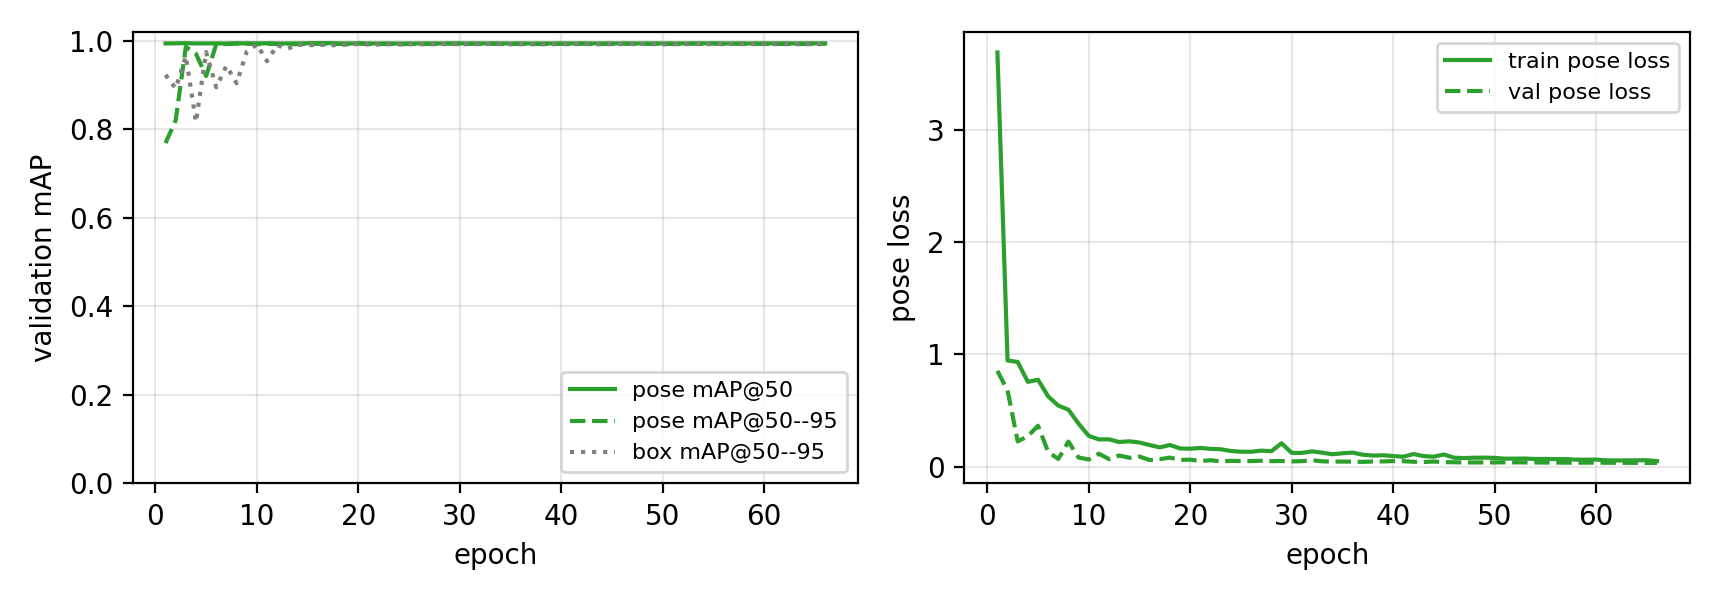
\includegraphics[width=0.92\textwidth]{04-CourtTrainingCurves.png}
	\caption{Training of the court keypoint model (YOLO26-pose, 66 epochs on a Colab T4 GPU). Left: validation mAP per epoch (pose mAP@50 solid, pose mAP@50--95 dashed, box mAP@50--95 dotted). Right: pose loss on the training (solid) and validation (dashed) splits.}
	\label{fig:court_curves}
\end{figure*}

	Figure~\ref{fig:ball_curves} shows the validation metrics of the two ball detectors during fine-tuning. Both converge smoothly within the 100 epochs, with mAP@50 saturating around epoch 60--70 while mAP@50--95 keeps improving slowly, consistent with the localization-bound regime discussed below. Table~\ref{tab:results} compares the two fine-tuned ball detectors against their zero-shot baselines on the test split.

\begin{figure*}[t]
	\centering
	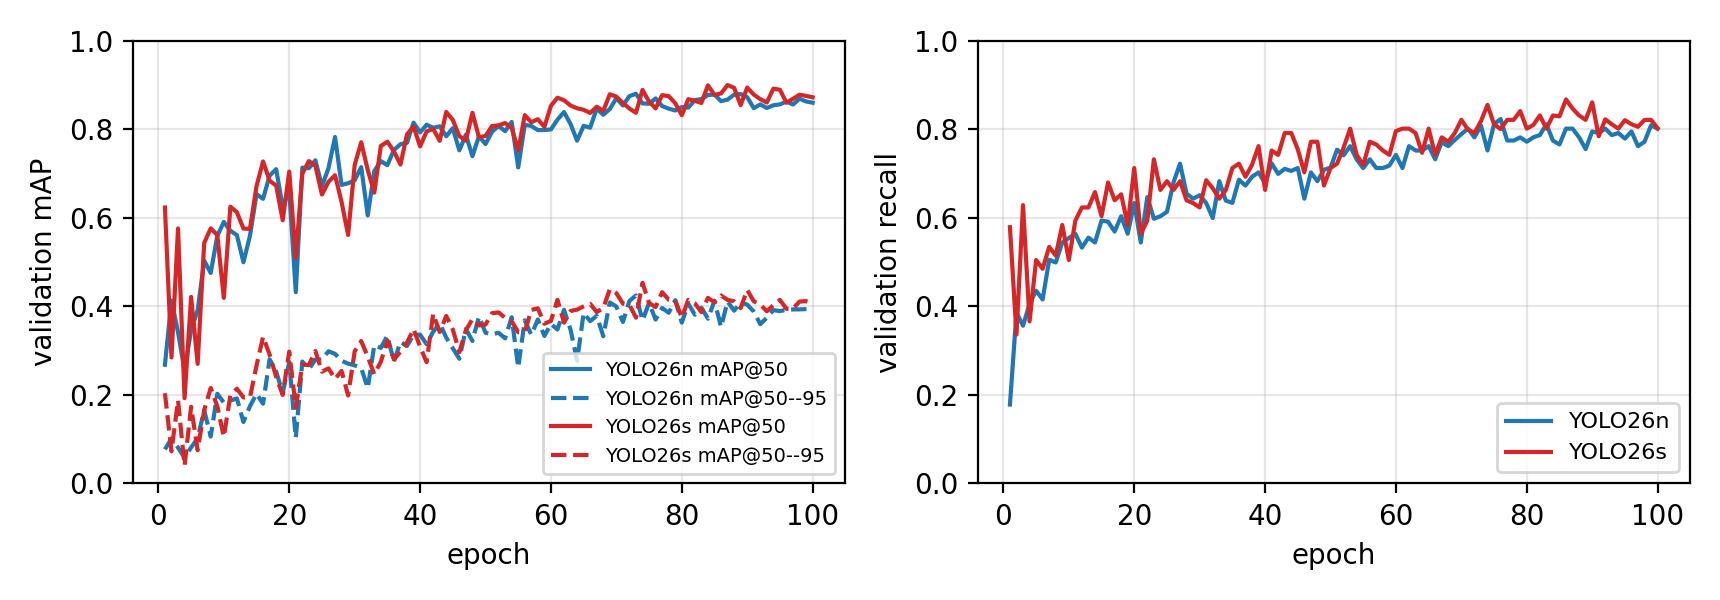
\includegraphics[width=0.92\textwidth]{03-BallTrainingCurves.png}
	\caption{Fine-tuning of the two ball detectors on the validation split. Left: mAP@50 (solid) and mAP@50--95 (dashed) per epoch. Right: recall per epoch. YOLO26s (red) consistently edges out YOLO26n (blue) at equal training settings.}
	\label{fig:ball_curves}
\end{figure*}

	The zero-shot baseline is the same COCO-pretrained checkpoint evaluated before any fine-tuning, restricted to the \emph{sports ball} class: it reaches at most $0.200$ mAP@50 and $0.320$ recall (YOLO26s), which quantifies how poorly the generic class transfers to broadcast tennis footage, where the ball is far smaller and blurrier than typical COCO instances. Fine-tuning on 428 images lifts mAP@50 by $+0.70$ and recall by $+0.56$ for the same architecture. Both fine-tuned variants reach high detection quality; YOLO26s outperforms YOLO26n on every quality metric on the test set (mAP@50 $0.905$ vs.\ $0.860$, recall $0.880$ vs.\ $0.805$) at the cost of roughly $45\%$ slower inference ($17.8$ vs.\ $12.3$ ms/image). The moderate mAP@50--95 values ($\approx 0.44$--$0.49$) are expected for an object only a few pixels wide: at tight IoU thresholds even a one-pixel localization error is penalized, while for the downstream pipeline (trajectory smoothing in continuous coordinates) mAP@50-level localization is sufficient.

	\begin{table}[h]
		\centering
		\caption{Ball detection on the test split: COCO zero-shot baselines (\emph{sports ball} class) vs.\ fine-tuned models.}
		\label{tab:results}
		\begin{tabular}{|l|c|c|c|}
			\hline
			\textbf{Method} & \textbf{mAP@50} & \textbf{Recall} & \textbf{Time} \\
			\hline
			YOLO26n zero-shot & 0.064 & 0.160 & -- \\
			YOLO26s zero-shot & 0.200 & 0.320 & -- \\
			\hline
			YOLO26n fine-tuned & 0.860 & 0.805 & 12.3 ms \\
			YOLO26s fine-tuned & 0.905 & 0.880 & 17.8 ms \\
			\hline
		\end{tabular}
	\end{table}

	The court keypoint model was evaluated on the 2211 held-out frames, reaching $0.994$ pose mAP@50 and $0.994$ pose mAP@50--95 (box mAP@50 $0.994$, pose precision $0.997$, recall $0.995$, $5.2$ ms/image). The training curves in Fig.~\ref{fig:court_curves} (66 epochs) show that the pose mAP saturates near $0.99$ within the first ten epochs and the validation loss tracks the training loss closely throughout, with no sign of overfitting -- confirming that court keypoint regression on a static broadcast view is an essentially solved sub-problem given enough training data.

	Qualitatively, the estimated homography projects the players and the smoothed ball track onto the minimap consistently across rallies, and the detected shots coincide with the visible hits in the annotated output videos. The rendered confidence labels also make the pipeline inspectable at a glance: frames where the ball marker carries no confidence value are exactly those bridged by the parabolic fit rather than detected, so the share of interpolated frames is directly visible in the output.

	\subsection{Critical Discussion}

	The comparison between the two ball variants shows a genuine capacity effect: YOLO26s improves recall by 7.5 points on the test set, which matters directly for the pipeline, since every missed detection widens the gaps the parabolic smoother must bridge. YOLO26n trades this for faster inference; given that the pipeline runs offline, YOLO26s is the better default, while YOLO26n remains a valid choice for near-real-time use.

	The fine-tuning itself is clearly beneficial, and Table~\ref{tab:results} quantifies it: the pretrained COCO \emph{sports ball} class recovers less than a third of the balls (recall $0.320$ at best), so no amount of downstream smoothing could compensate for the missing detections. The hardest conditions for the ball detector are fast serves and shots near the players' bodies, where motion blur stretches the ball into a faint streak; these are exactly the frames the smoother is designed to recover by interpolating within a parabolic segment. The main failure modes of the full pipeline are: rallies with very long detection gaps, where no parabolic segment can be fit and shot speeds become unavailable; and shots with little displacement along the court length (e.g.\ sharp cross-court angles), which weaken the velocity-reversal signal used for hit detection. Camera cuts and replays are instead handled explicitly: the per-frame court classification masks out non-court frames, the parabolic fit is prevented from bridging cuts, and player selection is repeated per court-visible segment.

	These observations are coherent with the related work: as in TrackNet~\cite{huang2019tracknet}, the bottleneck is small-object detection under motion blur rather than association or geometry. The main limitations of the project are the moderate size of the ball dataset, the single-camera setup (no ball height, so reported shot speeds are projections on the court plane), and the heuristic nature of the event rules, whose thresholds are tuned on broadcast footage.

	\section{Conclusion}

	This project addressed the extraction of quantitative match statistics from single-camera broadcast tennis videos. A complete pipeline was built around three YOLO26 models: a custom-trained court keypoint pose model, a pretrained player tracker, and a ball detector fine-tuned on a dedicated dataset, with all analytics computed in metric court coordinates via homography. Experimentally, the fine-tuned YOLO26s ball detector reached 0.905 mAP@50 and 0.880 recall on a held-out test set, outperforming the nano variant at a modest inference cost, and the court model was validated on 2211 unseen frames. The student's contributions span dataset preparation, model training, a physics-motivated trajectory smoother, metric shot and bounce detection, and the integration of the full system. The main limitations are the planar speed estimates inherent to the single-camera setup and the sensitivity to long ball-detection gaps.

	\section*{Acknowledgments}

	The project uses the Ultralytics YOLO framework and PyTorch. The court keypoint model was trained on Google Colab (NVIDIA T4 GPU).

	\bibliographystyle{ieeetr}
	\bibliography{references}

\end{document}
